In the second semester, we focused our evaluation on the CREMI dataset. Only
one volume was used for the training, which has a size of $1250\times 1250\times 125$.\\
To get an even bigger dataset for the training, we used data augmentation with
elastic transformations, modification of the brightness and contrast, and also vertical and horizontal flip, like in the paper.\\

One thing that was an issue during the first semester that we wanted to fix was
the segmentation of the nuclei, we were not able to include it clearly in the
cell due to the small patch size, but this should be alleviated with the
unet.\\

An issue for evaluation is that we were not able to create an account tu
evaluate our model on the test set, so we had to improvise our test set.
As we have seen, we are not predicting in 3D, so we’ll comsider our dataset as 125 images of size $1250\times 1250$.\\ 
We’ll split the dataset in 100 images for the training and 25 images for the testing.\\

For the post processing, we will just average the edge weights as
in~\cite{funke_large_2019} but we will only do a watershed to obtain our
segmentation, as it gave us the best results from what we tried.

\begin{figure}[!htbp]
    \centering
    \begin{subfigure}[t]{0.31\textwidth}
        \centering
        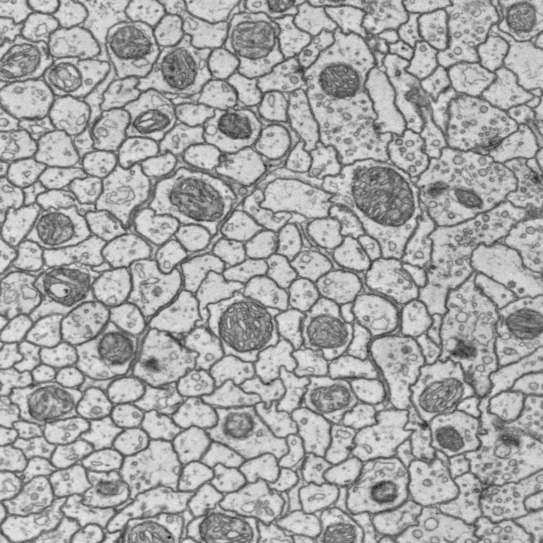
\includegraphics[height=0.9\textwidth]{./images/results/raw_1.png}
        \caption{Original image}
    \end{subfigure}%
    \begin{subfigure}[t]{0.31\textwidth}
        \centering
        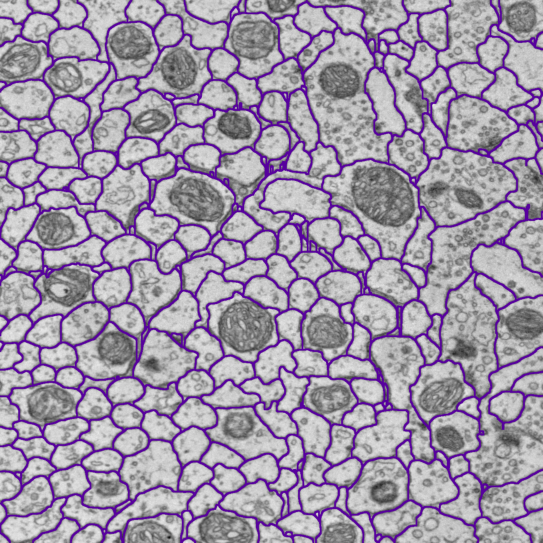
\includegraphics[height=0.9\textwidth]{./images/results/pred_1.png}
        \caption{Our segmentation}
    \end{subfigure}%
    \begin{subfigure}[t]{0.31\textwidth}
        \centering
        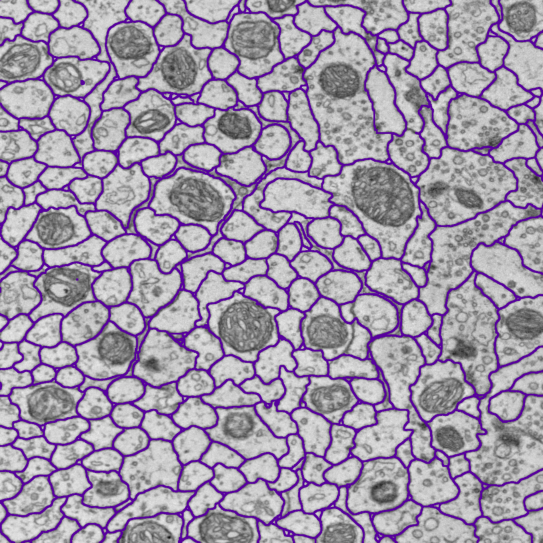
\includegraphics[height=0.9\textwidth]{./images/results/gt_1.png}
        \caption{Groundtruth}
    \end{subfigure}
	\caption{Results on the CREMI dataset volume A. We represented borders
	around cells instead of labels for more clarity.}
	\label{fig:cremi_results_s2_a}
\end{figure}


As we can see in figure~\ref{fig:cremi_results_s2_a} our results are very good
since our segmentation is rather close to the groundtruth and most cells are well separated.
Even the nucleus were taking into account in the segmentation, which is what we
were aiming for.\\
However there are still some missing boundaries which can cause the fusion of two cells.\\
We provide more examples of results in annex.\\

We evaluated our results with several metrics :
\begin{itemize}
  \item the Rand Index
  \item the Variation of Information (VOI) merge and split
  \item the CREMI score.
\end{itemize}

The Rand Index, as we talked earlier is defined as :\\
\begin{gather*}
	1 - RI(\hat{S},S) = \binom{N}{2}^{-1} \sum_{i<j} \lvert \delta(s_i,s_j) -
	\delta(\hat{s}_i,\hat{s}_j) \rvert
\end{gather*}
It should be closer to 1 to be better\\

The Variation of Information (VOI) is determined by :\\
\begin{gather*}
	VOI(\hat{S},S) = H(\hat{S}|S) + H(S|\hat{S})
\end{gather*}
Here $S$ is our groundtruth segmentation and $\hat{S}$ our predicted segmentation.
The conditional entropy $H(\hat{S}|S)$ corresponding to the VOI split, can be interpreted as the amount of over-segmentation.\\
Likewise, the conditional entropy $H(S|\hat{S})$ corresponding to the VOI merge, is the amount of under-segmentation.\\
In other word, a perfect over-segmentation will have $H(S|\hat{S}) = 0$ and a perfect under-segmentation will have $H(\hat{S}|S) = 0$.\\
The VOI should be lower to be better.\\

The CREMI score corresponds to the geometric mean of the $VOI(\hat{S},S)$ and $1-R(\hat{S},S)$ such as :\\
\begin{gather*}
	CREMI = \sqrt{VOI(\hat{S},S)\times (1 - R(\hat{S},S))}
\end{gather*}
It is the score used to rank submissions to the leaderboard. It also should be lower to be better.\\

\begin{table}[!htbp]
	\centering
	\begin{tabular}{|c|c|c|c|c|}
		\hline
		& Rand index & \thead{VOI merge \\(lower is better)} & \thead{VOI split\\(lower is better)} & \thead{CREMI score\\(lower is better)}\\
		\hline
		FCN + MALIS & 0.61 & 1.25 & 1.03 & 0.94\\
		\hline
		U-net & 0.58 & 0.91 & \textbf{0.52} & 0.78\\
		\hline
		U-net MALA & \textbf{0.83} & \textbf{0.46} & 0.54 & \textbf{0.42}\\
		\hline
	\end{tabular}
	\caption{Results on the training set of the CREMI dataset}
\label{tab:cremi_res_train}
\end{table}
\begin{table}[!htbp]
	\centering
	\begin{tabular}{|c|c|c|c|c|}
		\hline
		& Rand index & \thead{VOI merge \\(lower is better)} & \thead{VOI split\\(lower is better)} & \thead{CREMI score\\(lower is better)}\\
		\hline
		FCN + MALIS & 0.53 & 1.57 & 1.38 & 1.18\\
		\hline
		U-net & 0.52 & 1.07 & \textbf{0.47} & 0.87\\
		\hline
		U-net MALA & \textbf{0.80} & \textbf{0.50} & 0.57 & \textbf{0.46}\\
		\hline
		\hline
		\textit{SOTA (in 3D)} & \textit{0.89} & \textit{0.115} & \textit{0.339}& \textit{0.221}\\
		\hline
	\end{tabular}
	\caption{Results on the test set of the CREMI dataset}
\label{tab:cremi_res_test}
\end{table}

Our numerical results on the training set can be seen on the table ~\ref{tab:cremi_res_train}.\\
The FCN + MALIS is what is what we obtained after implementing the first paper.
The U-net is just a U-Net with a BCE loss.
Finally the U-net MALA is a U-net with the constrained MALIS loss (the improves
version of MALIS), both this and the U-Net had the same post processing.\\

For the training set, we get a Rand Index of 0.83 for the U-net MALA which is much higher than the simple U-net with a rand index of 0.58, and also higher than the Rand index of 0.61 we get with the FCN.\\
The U-net MALA has the lowest VOI merge by far while the FCN have the highest. The VOI split are quite the same for the U-net and U-net MALA.\\
However it is good to note that there is kind of a tradeoff between the VOI merge and VOI split, and as such comparing the sum is a better indicator.\\
Our U-net MALA has the best CREMI score of 0.42 compared to the simple U-net and the FCN.\\ 
We can see that our U-net MALA has the best results on the training set, and we
will see if it generalizes well on our test set.\\

Just like the training set, our numerical results for the test set are shown in the table~\ref{tab:cremi_res_test}.\\
As we can see, the results with the U-Net MALA are quite similar to what we had before, thanks in part to the data augmentation that allows it to be more robust.\\
As before, our CREMI score is much lower when compared to the U-Net, which is to be expected, and a good indicator of success.\\

However as you can see we are still far from the state of the art, especially for the VOI. One thing that could cause this is the different post processing used.\\ 
Indeed we did not have the time to implement the same post processign that was
used in~\cite{funke_large_2019}, and our implementation was painfully slow, so
we didn't use it.\\
However, we can’t really compare our results with the state of the art because it’s in 3D and we’re predicting in 2D which causes us to use less information when predicting.\\
Yet the results we obtained, although not state of the art, still demonstrates
well that the MALIS method can improve results in a significant manner.\\
